\documentclass[man]{apa6}

\usepackage{amssymb,amsmath}
\usepackage{ifxetex,ifluatex}
\usepackage{fixltx2e} % provides \textsubscript
\ifnum 0\ifxetex 1\fi\ifluatex 1\fi=0 % if pdftex
  \usepackage[T1]{fontenc}
  \usepackage[utf8]{inputenc}
\else % if luatex or xelatex
  \ifxetex
    \usepackage{mathspec}
    \usepackage{xltxtra,xunicode}
  \else
    \usepackage{fontspec}
  \fi
  \defaultfontfeatures{Mapping=tex-text,Scale=MatchLowercase}
  \newcommand{\euro}{€}
\fi
% use upquote if available, for straight quotes in verbatim environments
\IfFileExists{upquote.sty}{\usepackage{upquote}}{}
% use microtype if available
\IfFileExists{microtype.sty}{\usepackage{microtype}}{}

% Table formatting
\usepackage{longtable, booktabs}
\usepackage{lscape}
% \usepackage[counterclockwise]{rotating}   % Landscape page setup for large tables
\usepackage{multirow}		% Table styling
\usepackage{tabularx}		% Control Column width
\usepackage[flushleft]{threeparttable}	% Allows for three part tables with a specified notes section
\usepackage{threeparttablex}            % Lets threeparttable work with longtable

% Create new environments so endfloat can handle them
% \newenvironment{ltable}
%   {\begin{landscape}\begin{center}\begin{threeparttable}}
%   {\end{threeparttable}\end{center}\end{landscape}}

\newenvironment{lltable}
  {\begin{landscape}\begin{center}\begin{ThreePartTable}}
  {\end{ThreePartTable}\end{center}\end{landscape}}

  \usepackage{ifthen} % Only add declarations when endfloat package is loaded
  \ifthenelse{\equal{\string man}{\string man}}{%
   \DeclareDelayedFloatFlavor{ThreePartTable}{table} % Make endfloat play with longtable
   % \DeclareDelayedFloatFlavor{ltable}{table} % Make endfloat play with lscape
   \DeclareDelayedFloatFlavor{lltable}{table} % Make endfloat play with lscape & longtable
  }{}%



% The following enables adjusting longtable caption width to table width
% Solution found at http://golatex.de/longtable-mit-caption-so-breit-wie-die-tabelle-t15767.html
\makeatletter
\newcommand\LastLTentrywidth{1em}
\newlength\longtablewidth
\setlength{\longtablewidth}{1in}
\newcommand\getlongtablewidth{%
 \begingroup
  \ifcsname LT@\roman{LT@tables}\endcsname
  \global\longtablewidth=0pt
  \renewcommand\LT@entry[2]{\global\advance\longtablewidth by ##2\relax\gdef\LastLTentrywidth{##2}}%
  \@nameuse{LT@\roman{LT@tables}}%
  \fi
\endgroup}


  \usepackage{graphicx}
  \makeatletter
  \def\maxwidth{\ifdim\Gin@nat@width>\linewidth\linewidth\else\Gin@nat@width\fi}
  \def\maxheight{\ifdim\Gin@nat@height>\textheight\textheight\else\Gin@nat@height\fi}
  \makeatother
  % Scale images if necessary, so that they will not overflow the page
  % margins by default, and it is still possible to overwrite the defaults
  % using explicit options in \includegraphics[width, height, ...]{}
  \setkeys{Gin}{width=\maxwidth,height=\maxheight,keepaspectratio}
\ifxetex
  \usepackage[setpagesize=false, % page size defined by xetex
              unicode=false, % unicode breaks when used with xetex
              xetex]{hyperref}
\else
  \usepackage[unicode=true]{hyperref}
\fi
\hypersetup{breaklinks=true,
            pdfauthor={},
            pdftitle={Measuring Lay Theories of Parenting and Child Development},
            colorlinks=true,
            citecolor=blue,
            urlcolor=blue,
            linkcolor=black,
            pdfborder={0 0 0}}
\urlstyle{same}  % don't use monospace font for urls

\setlength{\parindent}{0pt}
%\setlength{\parskip}{0pt plus 0pt minus 0pt}

\setlength{\emergencystretch}{3em}  % prevent overfull lines


% Manuscript styling
\captionsetup{font=singlespacing,justification=justified}
\usepackage{csquotes}
\usepackage{upgreek}



\usepackage{tikz} % Variable definition to generate author note

% fix for \tightlist problem in pandoc 1.14
\providecommand{\tightlist}{%
  \setlength{\itemsep}{0pt}\setlength{\parskip}{0pt}}

% Essential manuscript parts
  \title{Measuring Lay Theories of Parenting and Child Development}

  \shorttitle{Measuring Parenting Theories}


  \author{Emily Hembacher\textsuperscript{1}~\& Michael C. Frank\textsuperscript{1}}

  % \def\affdep{{"", ""}}%
  % \def\affcity{{"", ""}}%

  \affiliation{
    \vspace{0.5cm}
          \textsuperscript{1} Stanford University  }

  \authornote{
    Add complete departmental affiliations for each author here. Each new
    line herein must be indented, like this line. Enter author note here.
    
    Correspondence concerning this article should be addressed to Michael C.
    Frank, 450 Serra Mall, Stanford, CA 94301. E-mail:
    \href{mailto:mcfrank@stanford.edu}{\nolinkurl{mcfrank@stanford.edu}}
  }


  \abstract{Enter abstract here. Each new line herein must be indented, like this
line.}
  \keywords{keywords \\

    \indent Word count: X
  }





\usepackage{amsthm}
\newtheorem{theorem}{Theorem}[section]
\newtheorem{lemma}{Lemma}[section]
\theoremstyle{definition}
\newtheorem{definition}{Definition}[section]
\newtheorem{corollary}{Corollary}[section]
\newtheorem{proposition}{Proposition}[section]
\theoremstyle{definition}
\newtheorem{example}{Example}[section]
\theoremstyle{definition}
\newtheorem{exercise}{Exercise}[section]
\theoremstyle{remark}
\newtheorem*{remark}{Remark}
\newtheorem*{solution}{Solution}
\begin{document}

\maketitle

\setcounter{secnumdepth}{0}



\section{Survey Construction}\label{survey-construction}

\subsection{Generation of items}\label{generation-of-items}

\subsection{Revised questionnaire
norming}\label{revised-questionnaire-norming}

\section{Survey Validation}\label{survey-validation}

\subsection{External Validity Study 1: Demographic
Factors}\label{external-validity-study-1-demographic-factors}

\begin{figure}
\centering
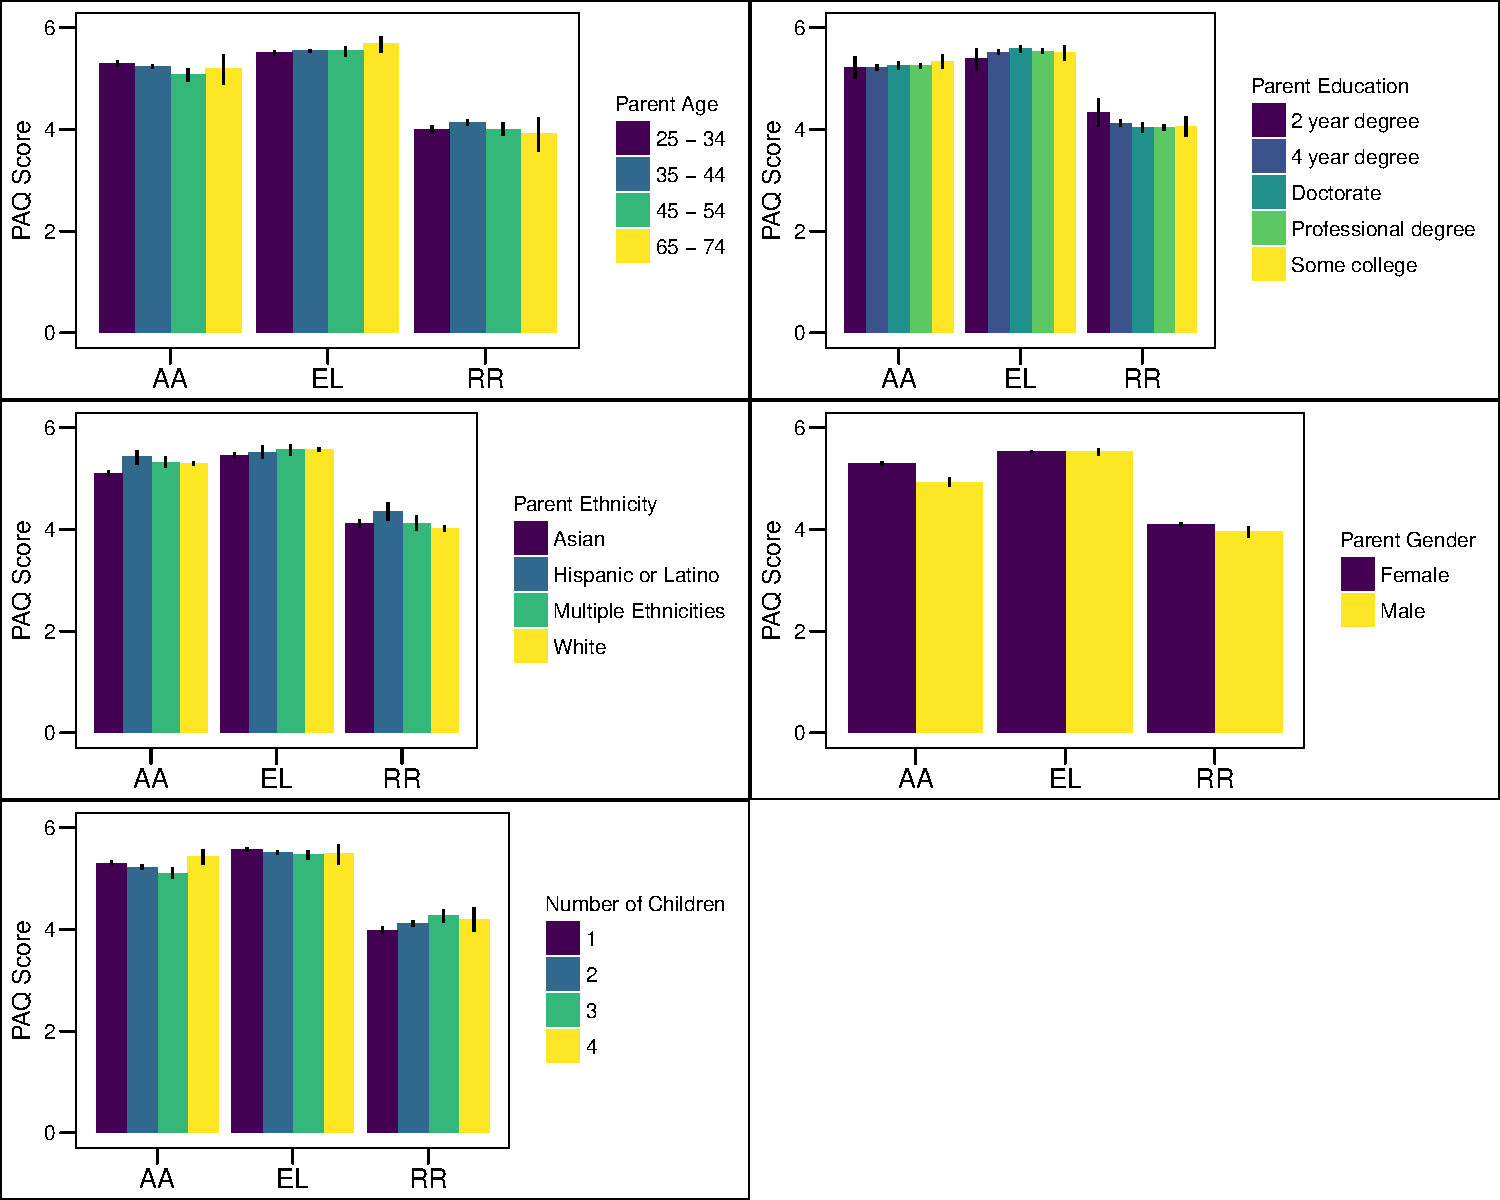
\includegraphics{PAQ_paper_files/figure-latex/demographics-1.pdf}
\caption{\label{fig:demographics}Demographic variability in PAQ scores.
Error bars represent +/-95\% CI computed by non-parametric bootstrap.}
\end{figure}

\begin{table}[h]
\centering
\caption{Results of separate bayesian ordinal logistic regressions of demographic factors on agreement with AA, EL, and RR attitudes.} 
\label{tab:demo}
\begin{tabular}{llrrrr}
  \hline
Subscale & Factor & Estimate & Est. Error & Lower 95\% CI & Upper 95\% CI \\ 
  \hline
AA & Parent Age & -0.00 & 0.01 & -0.01 & 0.01 \\ 
   & Hispanic or Latino & 0.72 & 0.20 & 0.34 & 1.11 \\ 
   & Multiple Ethnicities & 0.50 & 0.16 & 0.18 & 0.82 \\ 
   & White & 0.31 & 0.09 & 0.12 & 0.49 \\ 
   & Parent Education & 0.02 & 0.02 & -0.01 & 0.05 \\ 
   & Number of children & -0.14 & 0.05 & -0.24 & -0.03 \\ 
   & Male & -0.70 & 0.11 & -0.92 & -0.48 \\ 
   \hline
EL & Parent Age & 0.01 & 0.01 & -0.00 & 0.02 \\ 
   & Hispanic or Latino & 0.26 & 0.19 & -0.12 & 0.64 \\ 
   & Multiple Ethnicities & 0.56 & 0.17 & 0.22 & 0.90 \\ 
   & White & 0.44 & 0.09 & 0.25 & 0.62 \\ 
   & Parent Education & 0.02 & 0.02 & -0.01 & 0.05 \\ 
   & Number of children & -0.14 & 0.05 & -0.24 & -0.03 \\ 
   & Male & -0.18 & 0.11 & -0.41 & 0.04 \\ 
   \hline
RR & Parent Age & -0.00 & 0.01 & -0.01 & 0.01 \\ 
   & Hispanic or Latino & 0.27 & 0.20 & -0.11 & 0.67 \\ 
   & Multiple Ethnicities & -0.02 & 0.17 & -0.34 & 0.31 \\ 
   & White & -0.20 & 0.10 & -0.38 & -0.01 \\ 
   & Parent Education & -0.02 & 0.02 & -0.05 & 0.01 \\ 
   & Number of children & 0.15 & 0.06 & 0.04 & 0.25 \\ 
   & Male & -0.17 & 0.12 & -0.39 & 0.06 \\ 
   \hline
\end{tabular}
\end{table}

Approaches to parenting are known to differ across cultures and groups.
To better understand whether the parenting attitudes captured by our
survey reflect group differences, we examined average scores on the PAQ
subscales based on demographic factors. We administered the PAQ to 680
parents who were members of a local children's museum and subsequently
asked them to provide information about their gender, level of
education, age, ethnicity, and the number of children they have. Figure
\ref{fig:demographics} displays the average PAQ scores for each
demographic category.

To quantify any possible group differences, we fit separate Bayesian
mixed-effects ordinal regression models for each subscale (AA, EL, RR)
with the following structure, with likert ratings of agreement for each
item (1-6) entered as dependent measures:
\texttt{agreement\ rating\ \textasciitilde{}\ age\ +\ education\ +\ ethnicity\ +\ gender\ +\ number\ of\ children\ +\ (1\ \textbar{}\ subject)\ +\ (1\textbar{}\ item)}
Groups with fewer than 20 cases were removed from plots and analyses to
avoid overfitting. Although displayed as categorical for visual
simplicity in Figure \ref{fig:demographics}, parent age and education in
years were entered as continuous variables in the regression models.

Table \ref{tab:demo} displays the results of the regression analyses. We
found that stronger agreement with AA attitudes was associated with
identifying as Hispanic or Latino (\(\beta\) = 0.72, 95\% CI = 0.34 -
1.11), White (\(\beta\) = 0.31, 95\% CI = 0.12 - 0.49), or multiple
ethnicities (\(\beta\) = 0.50, 95\% CI = 0.18 - 0.82) compared to Asian
(the comparison level). Having a greater number of children was
associated with lower agreement with AA attitudes (\(\beta\) = -0.14,
95\% CI = -0.24 - -0.03), as was identifying as Male (\(\beta\) = -0.70,
95\% CI = -0.92 - -0.48). Parent education was not meaningfully
associated with AA scores.

We found that stronger agreement with EL scores was associated with
identifying as White (\(\beta\) = 0.44, 95\% CI = 0.25 - 0.62) or
multiple ethnicities (\(\beta\) = 0.56, 95\% CI = 0.22 - 0.90), and
having more children was associated with slightly lower agreement with
EL scores (\(\beta\) = -0.14, 95\% CI = -0.24 - -0.03). No other
demographic variables were related to EL scores.

Finally, we found that stronger agreement with RR attitudes was
associated with having a greater number of children (\(\beta\) = 0.15,
95\% CI = 0.04 - 0.25), and identifying as White was associated with
lower agreement with RR attitudes (\(\beta\) = -0.20, 95\% CI = -0.38 -
-0.01).

\subsection{Study 2: Relation to parenting
behaviors}\label{study-2-relation-to-parenting-behaviors}

\begin{figure}
\centering
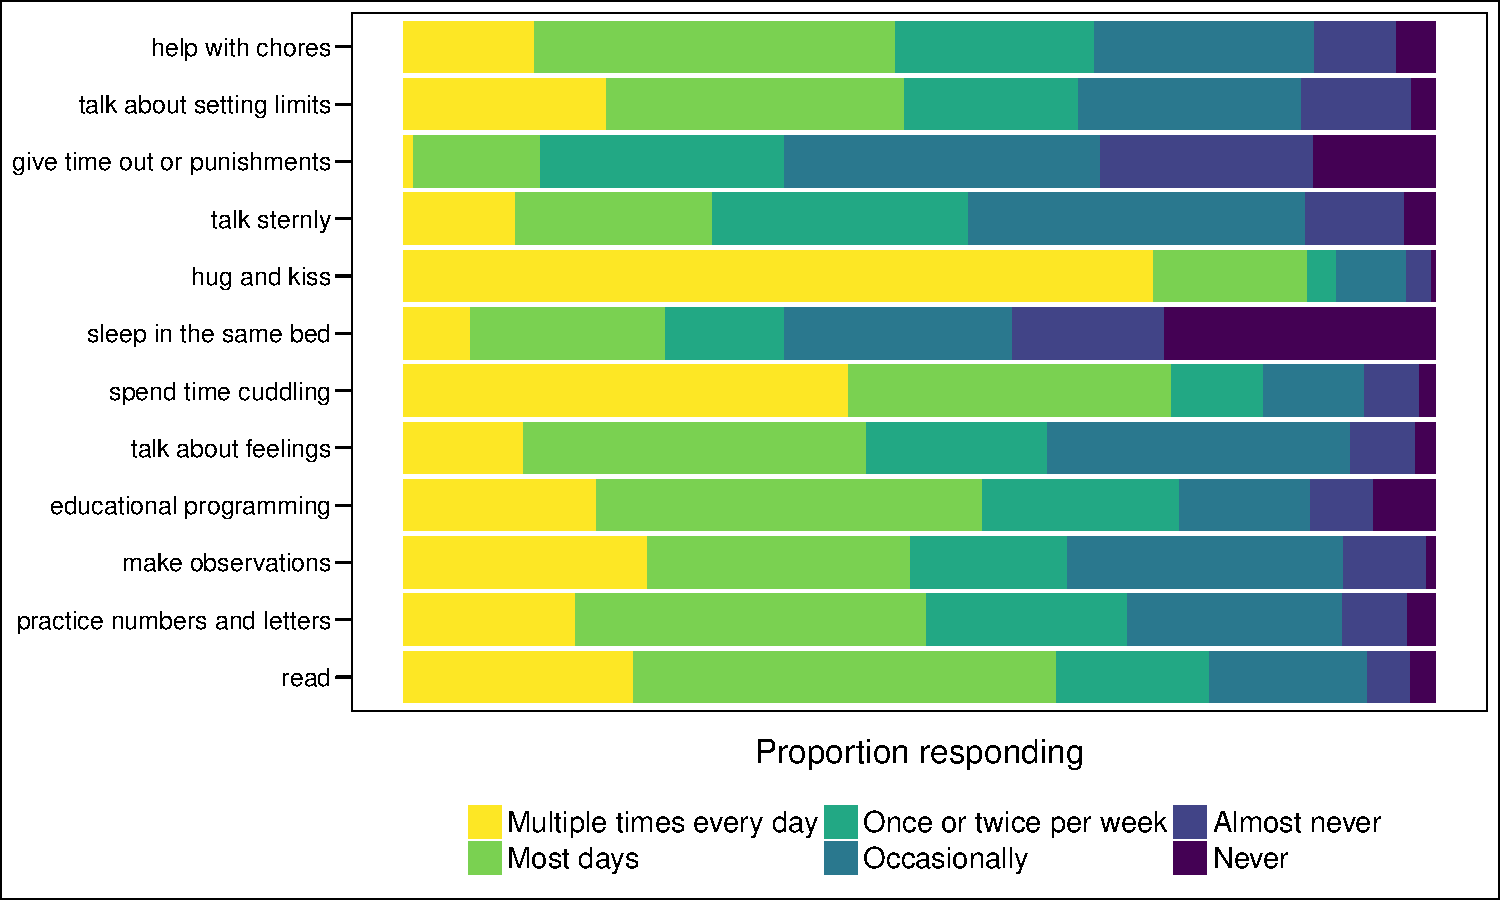
\includegraphics{PAQ_paper_files/figure-latex/behavefreq-1.pdf}
\caption{\label{fig:behavefreq}Frequencies of different parenting activities
reported by parents.}
\end{figure}

\begin{figure}
\centering
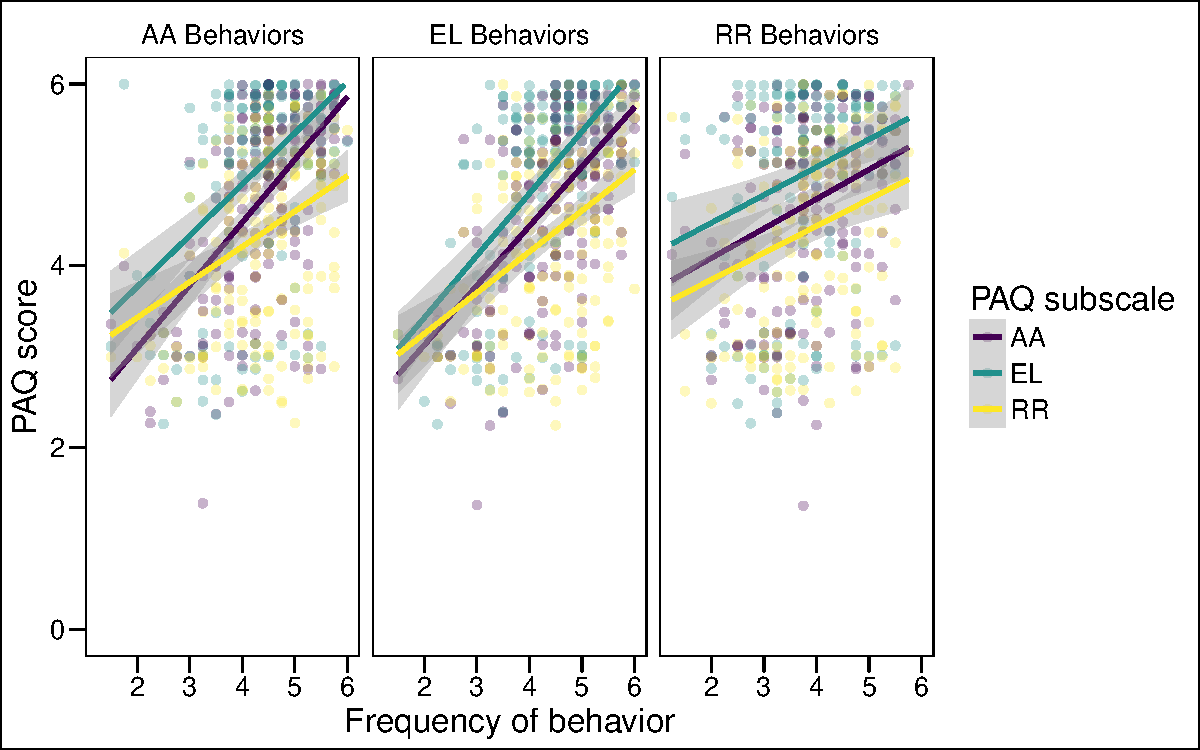
\includegraphics{PAQ_paper_files/figure-latex/behavepaq-1.pdf}
\caption{\label{fig:behavepaq}Relations between PAQ scores (Affection and
Attachment, Early Learning, and Rules and Respect) and the frequency of
parenting behaviors divided into the same categories.}
\end{figure}

\begin{table}[h]
\centering
\caption{Results of separate bayesian ordinal logistic regressions of PAQ scores and child age on frequency of parenting behaviors in Affection and Attachment (AA), Early Learning (EL), and Rules and Respect (RR) categories.} 
\label{tab:behavetab}
\begin{tabular}{llrrrr}
  \hline
Behavior Category & Factor & Estimate & Est. Error & Lower 95\% CI & Upper 95\% CI \\ 
  \hline
AA & AA PAQ score & 0.81 & 0.15 & 0.53 & 1.11 \\ 
   & RR PAQ score & -0.02 & 0.11 & -0.24 & 0.20 \\ 
   & EL PAQ score & -0.01 & 0.14 & -0.30 & 0.26 \\ 
   & Child Age & 0.01 & 0.01 & -0.00 & 0.02 \\ 
   \hline
EL & AA PAQ score & 0.36 & 0.18 & 0.01 & 0.73 \\ 
   & RR PAQ score & 0.20 & 0.14 & -0.07 & 0.47 \\ 
   & EL PAQ score & 0.52 & 0.18 & 0.17 & 0.88 \\ 
   & Child Age & 0.01 & 0.01 & -0.00 & 0.03 \\ 
   \hline
RR & AA PAQ score & 0.10 & 0.20 & -0.30 & 0.50 \\ 
   & RR PAQ score & 0.34 & 0.15 & 0.04 & 0.64 \\ 
   & EL PAQ score & 0.02 & 0.20 & -0.36 & 0.41 \\ 
   & Child Age & 0.03 & 0.01 & 0.01 & 0.05 \\ 
   \hline
\end{tabular}
\end{table}

\begin{table}

\caption{\label{tab:behavesents}Behaviors that parents were asked to report on, and their corresponding attitude categories.}
\centering
\begin{tabular}[t]{l|>{\raggedright\arraybackslash}p{35em}}
\hline
Category & In the last month, how often did...\\
\hline
AA & you and your child talk about feelings (e.g., when he/she was sad/angry)?\\
\hline
 & you and your child spend time cuddling?\\
\hline
 & your child sleep in the same bed as you?\\
\hline
 & you hug or kiss your child?\\
\hline
EL & you read to your child?\\
\hline
 & you practice numbers or letters with your child?\\
\hline
 & you share facts or observations about the world when you were doing other tasks (e.g., did you know butter comes from cows? while shopping at the grocery store)?\\
\hline
 & your child watch educational programming (e.g., shows like Sesame Street) or play with educational apps (e.g., apps designed to teach numbers, colors, shapes, etc.) on a tablet or mobile device?\\
\hline
RR & you talk sternly to your child when he/she did something you dont want?\\
\hline
 & you give your child time out or other punishments for acting out?\\
\hline
 & you talk about setting limits with your child (e.g., only 10 minutes of screen time or no hitting)?\\
\hline
 & your child help or try to help with chores or tasks (including cleaning up his/her toys)?\\
\hline
\end{tabular}
\end{table}

Another way of assessing the ecological validity of the PAQ is to ask
whether the parenting attitudes it assesses are related to actual
parenting behaviors. For example, do parents who strongly agree with
items on the Early Learning subscale read to their children more often?
Do parents who strongly endorse items on the Rules and Respect subscale
give more time-outs? To assess this, we asked a sample of 250 parents on
Amazon's Mechanical Turk to complete the PAQ and then rate the frequency
with which they engaged in a number of parenting behaviors, focusing on
the prior month (Table \ref{tab:behavesents}). We elicited responses
about 12 different behaviors, with four corresponding to each PAQ
category. Parents chose between the following frequency options:
\enquote{Multiple times per day}, \enquote{Most days}, \enquote{Once or
twice per week,} \enquote{Occasionally,} \enquote{Almost never,}
\enquote{Never,} and \enquote{My child is too young for this.} Parents
who did not have children under the age of 5 were excluded from
analyses, as were any responses of \enquote{My child is too young for
this.}

The distribution of frequencies that parents reported is displayed in
Figure \ref{fig:behavefreq}. To assess whether parenting behaviors are
associated with parenting attitudes, we calculated participants' average
PAQ subscale scores and fit separate bayesian ordinal logistic
mixed-effects regressions for the three cateogories of behaviors with
the following structure:
\texttt{behavior\ frequency\ \textasciitilde{}\ AA\ PAQ\ score\ +\ EL\ PAQ\ score\ +\ RR\ PAQ\ score\ +\ child\ age\ +\ (1\ \textbar{}\ subject)\ +\ (1\textbar{}\ item)}
(Table \ref{tab:behavetab}). The relation between PAQ scores and
behavior frequencies are presented in Figure \ref{fig:behavepaq}.

We found that the frequency of AA behaviors was positively associated
with AA attitudes (\(\beta\) = 0.81, 95\% CI = 0.53 - 1.11), but not RR
or EL attitudes or child age. Frequency of EL behaviors was positively
associated with stronger agreement with both AA (\(\beta\) = 0.36, 95\%
CI = 0.01 - 0.73) and EL attitudes (\(\beta\) = 0.52, 95\% CI = 0.17 -
0.88). The frequency of RR behaviors was positively associated with
stronger RR attitudes (\(\beta\) = 0.34, 95\% CI = 0.04 - 0.64), and to
a lesser extent, child age (\(\beta\) = 0.03, 95\% CI = 0.01 - 0.05).

\subsection{Study 3: Uptake of new information about parenting and child
development}\label{study-3-uptake-of-new-information-about-parenting-and-child-development}

Parents' attitudes about parenting and child development may be an
important consideration for crafting interventions on parenting
behaviors or beliefs. There are frequent efforts to intervene on
parenting practices, for example, public service announcements telling
parents to read to their children; courses aimed at helping fathers
engage with their children; messages aimed at encouraging parents and
teachers to give children opportunities for free play. There is evidence
that existing lay theories can interact in surprising ways with this
type of messaging in other domains. Here we asked whether parents'
attitudes about parenting and child development would predict how they
uptake new information about child development versus an unrelated
topic.

\begin{figure}
\centering
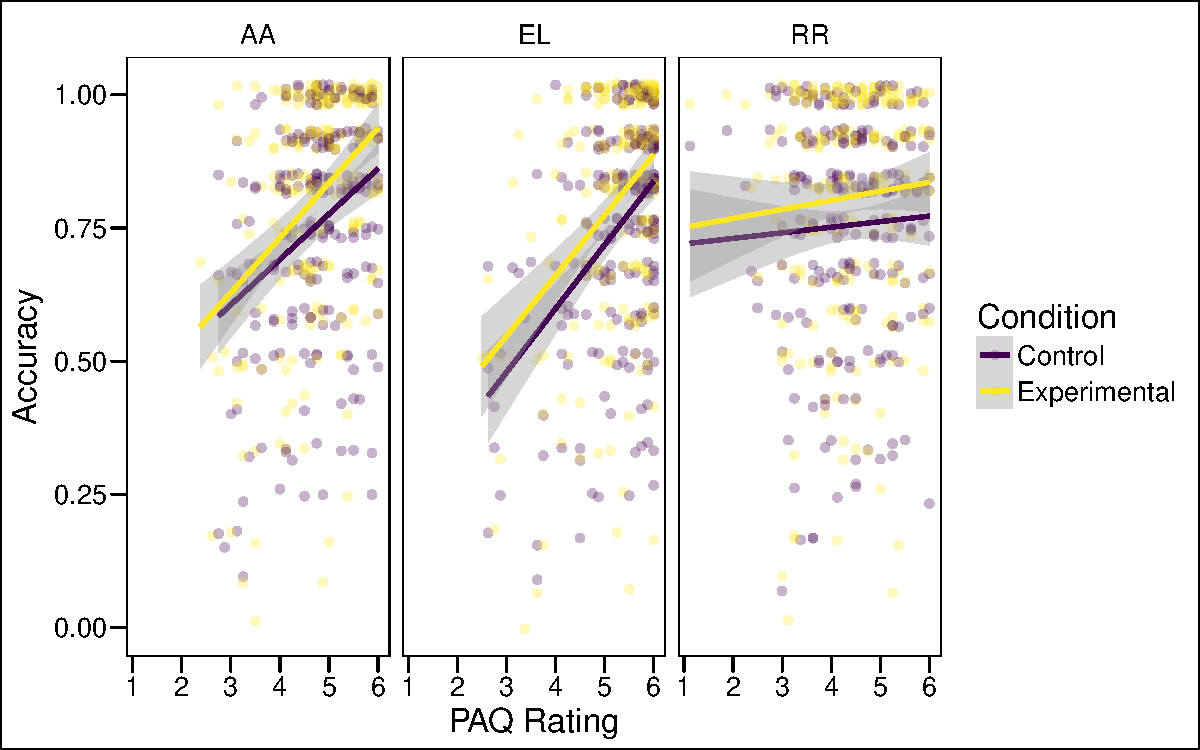
\includegraphics{PAQ_paper_files/figure-latex/uptake-1.pdf}
\caption{\label{fig:uptake}Relations between PAQ scores (Affection and
Attachment, Early Learning, and Rules and Respect) and the uptake of
information in experimental (child development-related) and control
articles.}
\end{figure}

\begin{table}[h]
\centering
\caption{Results of a bayesian logistic regression of PAQ scores and experimental condition on accuracy.} 
\label{tab:uptake}
\begin{tabular}{lrrrr}
  \hline
Factor & Estimate & Est. Error & Lower 95\% CI & Upper 95\% CI \\ 
  \hline
Child Development Articles & -0.21 & 0.75 & -1.68 & 1.29 \\ 
  AA PAQ score & 0.05 & 0.15 & -0.25 & 0.35 \\ 
  RR PAQ score & -0.21 & 0.11 & -0.42 & 0.01 \\ 
  EL PAQ score & 0.82 & 0.16 & 0.52 & 1.14 \\ 
  AA PAQ score * Child Development Articles & 0.42 & 0.16 & 0.11 & 0.73 \\ 
  RR PAQ score * Child Development Articles & 0.02 & 0.11 & -0.19 & 0.23 \\ 
  EL PAQ score * Child Development Articles & -0.27 & 0.16 & -0.58 & 0.05 \\ 
   \hline
\end{tabular}
\end{table}

We asked 250 adults on Amazon's Mechanical Turk to fill out the PAQ and
then read four popular press articles, two of which related to child
development and two of which related to other science topics. The
articles were edited for length, and the order in which the articles
were presented was randomized. Next, participants answered six
four-alternative forced-choice questions testing their memory and
understanding of each article (24 total questions). We were specifically
interested in whether participants who agreed more strongly with EL
attitudes would better understand and remember the information in the
child development articles, which we predicted may have been consistent
with their existing views of development. Participants' accuracy in
relation to their average AA, EL and RR scores is displayed in Figure
\ref{fig:uptake}.

The average accuracy for control questions was 0.76(CI = 0.73 - 0.78)
and the average accuracy for experimenter questions was 0.81(CI = 0.73 -
0.84). There was no significant difference in accuracy between
conditions, t = -4.83, p = 0.00.

To assess whether participants who more strongly agreed with EL
attitudes were at an advantage for understanding and remembering the
child development articles they read, we fit a bayesian logistic
mixed-effects regression with the following structure:
\texttt{accuracy\ \textasciitilde{}\ AA\ PAQ\ score\ *\ article\ type\ +\ EL\ PAQ\ score\ *\ article\ type\ +\ RR\ PAQ\ score\ *\ article\ type\ +\ (article\ type\ \textbar{}\ subject)\ +\ (1\textbar{}\ item)}.
We excluded 7.70\% of responses from analyses because participants spent
fewer than 15 seconds reading the article, our pre-determined minimum
reading time.

We found that participants who agreed more strongly with EL attitudes
were more likely to answer uptake questions correctly overall (\(\beta\)
= 0.82, 95\% CI = 0.52 - 1.14), but there was no interaction between EL
scores and article type, meaning that there was no advantage for people
with higher EL scores for understanding child development content in
particular. However, unexpectedly, there was an interaction between AA
attitudes and article type (\(\beta\) = 0.42, 95\% CI = 0.11 - 0.73),
such that people with stronger AA attitudes performed better on
questions about child development articles compared to control articles.

\newpage

\section{References}\label{references}

\begingroup
\setlength{\parindent}{-0.5in} \setlength{\leftskip}{0.5in}

\hypertarget{refs}{}

\endgroup






\end{document}
